% Design Decisions
\section{Architecture}

\frame{
\frametitle{Pairwise Testing}
\begin{figure}
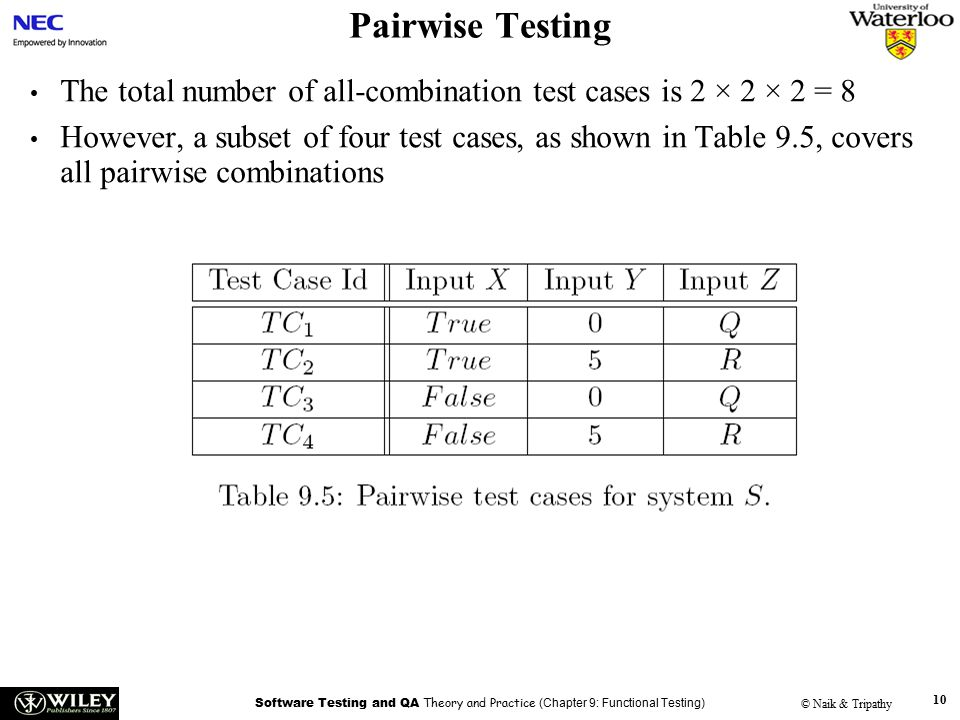
\includegraphics[scale=0.4]{pairwise.jpg}
\end{figure}
}

\frame{
\frametitle{ParmGen}
\begin{table}
\begin{tabular}{l | c | c}
\emph{Item Purchased} & \emph{Price} & \emph{Delivery Method} \\
\hline \hline
{\color{red}Large Item} & {\color{red}Expensive} & Lightspeed \\ 
Small Item & Mid-price & SnailMail \\
ExtraSmall Item & Cheap & {\color{red}Ultrafast} \\
\end{tabular}
\caption{Possibilities}
\end{table}

\begin{table}
\begin{tabular}{l | c | c}
\emph{Item Purchased} & \emph{Price} & \emph{Delivery Method} \\
\hline \hline
Boat & \$10,000.00 & Space Rocket \\
\end{tabular}
\caption{Concrete Test Vector}
\end{table}
}

\frame{
\frametitle{ParmGen Space}
\begin{columns}
    \begin{column}{0.48\textwidth}
        \begin{table}
        \begin{tabular}{l | c}
        \emph{Cats} & \emph{Dogs} \\
        \hline \hline
        10 & 1 \\
        \end{tabular}
        \caption{Unit Parameter}
        \end{table}
    \end{column}
    \begin{column}{0.48\textwidth}
        \begin{table}
        \begin{tabular}{l | c}
        \emph{Cats} &  \emph{Dogs}\\
        \hline \hline
        10 & 1 \\ 
        1 & 1 \\ 
        10 & 10 \\ 
        10 & 100 \\ 
        10 & 1 \\ 
        1 & 10 \\ 
        10 & 10 \\ 
        10 & 1 \\ 
        1 & 1 \\
        10 & 100 \\
        100 & 1 \\
        1 & 10 \\

        \end{tabular}
        \caption{System Parameter}
        \end{table}
    \end{column}
\end{columns}
}

\frame{
\frametitle{ParmGen Space}
Cats is \emph{not} just 100. \\
\vspace{1cm}
Cats is [10, 1, 10, 10, 10, 1, 10, 10, 1, 10, 100, 1, ...] \\
\pause
\vspace{1cm}
Cats is [1, 2, 2, 3, 3, 3, 4, 3, 2, 1, 1]
}


\frame{
\frametitle{100 points -- average $=$ 15, std. deviation $=$ 5}
\begin{figure}
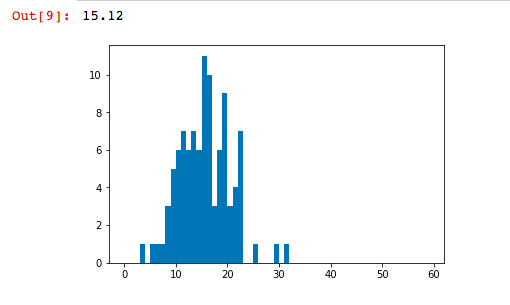
\includegraphics[scale=0.6]{law1.png}
\end{figure}
}

\frame{
\frametitle{Law of Large Numbers}
\begin{itemize}
\item Bernoulli's Principle
\item Selection Scheme
\end{itemize}
}

\frame{
\frametitle{10,000 points -- average $=$ 15, std. deviation $=$ 5}
\begin{figure}
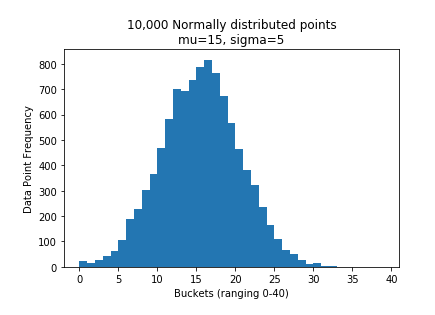
\includegraphics[scale=0.6]{law2.png}
\end{figure}
}

\frame{
\frametitle{300 points -- average $=$ 15, std. deviation $=$ 5}
\begin{figure}
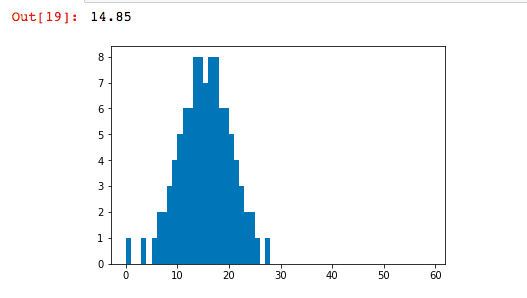
\includegraphics[scale=0.6]{law3.png}
\end{figure}
}

\frame{
\frametitle{A Variety of Statistical Distributions}
\begin{figure}
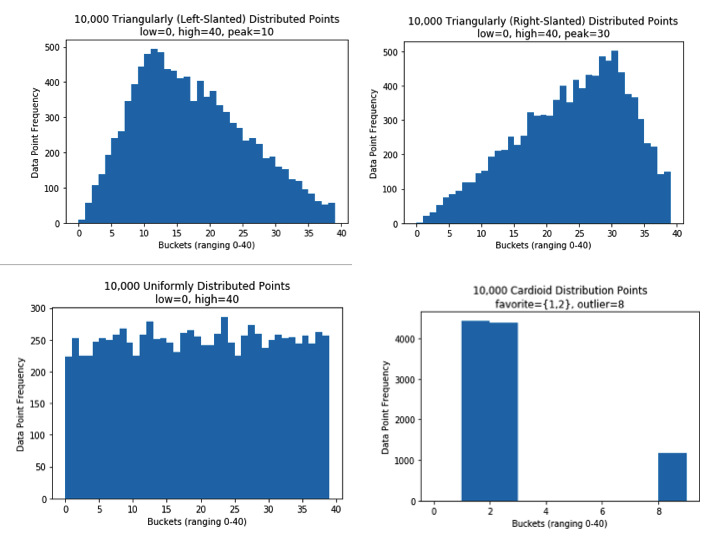
\includegraphics[scale=0.4]{distributions.png}
\end{figure}
}

\frame{
\frametitle{Cardioids}
$$r = \alpha \pm \alpha cos \theta$$
\begin{figure}
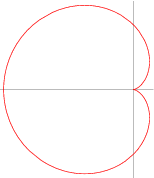
\includegraphics[scale=0.9]{cardioid.png}
\end{figure}
}

\frame{
\frametitle{Preprocessor}
\begin{figure}
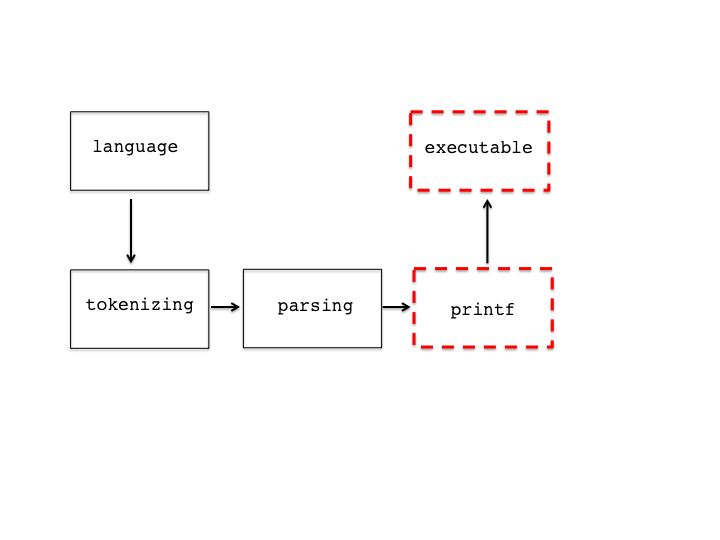
\includegraphics[scale=0.45]{preprocess.png}
\end{figure}
}

\frame{
\frametitle{GenSequence}
\begin{figure}
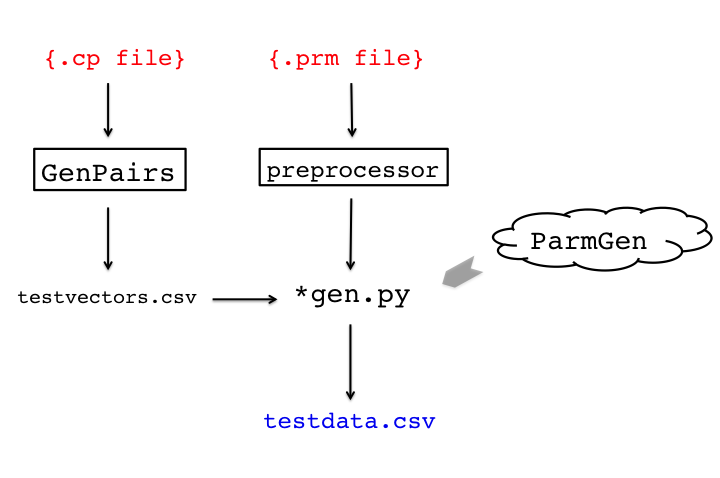
\includegraphics[scale=0.4]{workflow.png}
\end{figure}
}

\frame{
\frametitle{}
\begin{figure}
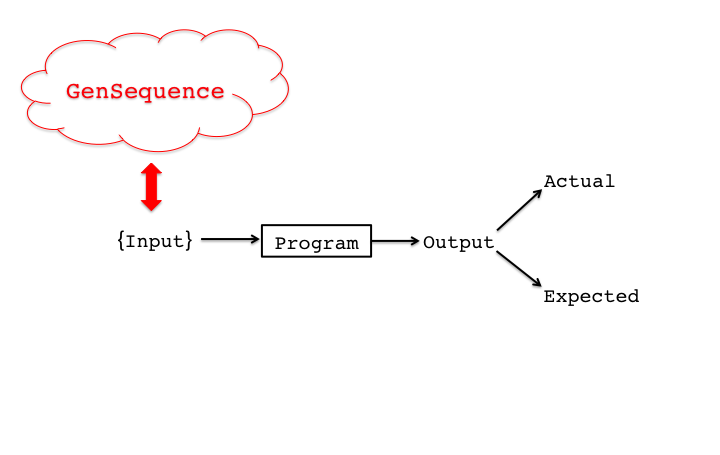
\includegraphics[scale=0.4]{diagram2.png}
\end{figure}
}